\section{Ход работы}

Объект защиты информации\cite{GOST50922} – информация или носитель информации, или информационный процесс, которые необходимо защищать в соответствии с целью защиты информации.

Объектами защиты будут являться:

\begin{itemize}
	\item Персональные данные сотрудников
	\item Бухгалтерская информация
	\item Номенклатура товаров
\end{itemize}	

\begin{figure}[H]
	\centering
	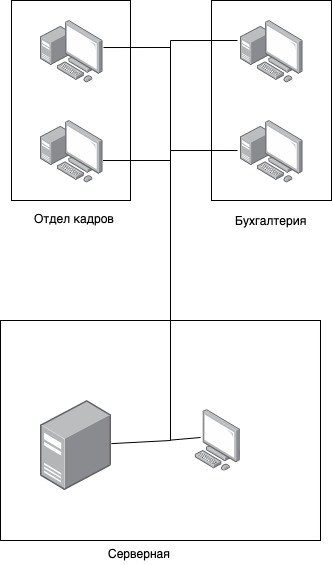
\includegraphics[width=.3\textwidth]{img/market.png}
	\caption{Схема подключения}
\end{figure}

Физическая защита информации\cite{GOST50922} - защита информации путем применения организационных мероприятий и совокупности средств, создающих препятствия для проникновения или доступа неуполномоченных физических лиц к объекту защиты

\begin{enumerate}
	\item Для обеспечения физической защиты помещений торговой фирмы необходима система контроля и управления доступом (СКУД), чтобы только сотрудники компании имели возможность с помощью электронных пропусков попасть внутрь служебных помещений. 
	\item Физический доступ в серверную должен быть доступен только ответственным сотрудникам торговой фирмы.
	\item Физическая защита персональных компьютеров сотрудников торговой фирмы достигается путем отключения внешних портов.
	\item Физический доступ в серверную ограничен еще одним специальным замком. Для доступа в помещение на смарт-карте должна быть дополнительная идентифицирующая информация, которая позволит получить доступ в серверную.
	\item Защита физического доступа к серверам обеспечивается наличием железной дверей, ведением журнала регистрации посещения серверного помещения, а также установкой системы видеонаблюдения для предотвращения несанкционированного доступа.
	\item Физическая защита персональных компьютеров сотрудников торговой фирмы обеспечивается использованием замков Kingston Lock.
\end{enumerate}

Логическая защита информации\cite{GOST50922} - защита информации, заключающаяся в обеспечении некриптографическими методами безопасности информации (данных), подлежащей (подлежащих) защите в соответствии с действующим законодательством, с применением технических, программных и программно-технических средств. 

\begin{enumerate}
	\item Для каждого сотрудника торговой фирмы создается отдельная учетная запись.
	\item Для доступа к персональным компьютерам применяется двухфакторая аутентификация.
	\item Для обеспечения высокой логической защиты на сервере и на компьютерах торговой фирмы должно быть установлено средство защиты информации, например, <<Dallas Lock>>, имеющий следующие функции:
	\begin{itemize}
		\item запрет загрузки компьютера посторонними лицам;
		\item 		двухфакторная авторизация по паролю и аппаратным идентификаторам (USB eToken, смарт-карты eToken, Rutoken, Touch Memory);
		\item 		разграничение прав пользователей на доступ к локальным и сетевым ресурсам;
		\item 		контроль работы пользователей со сменными накопителями;
		\item 		мандатный и дискреционный принципы разграничения прав;
		\item 		организация замкнутой программной среды;
		\item 		аудит действий пользователей;
		\item 		контроль целостности ресурсов компьютера;
		\item 		очистка остаточной информации;
		\item 		возможность автоматической печати штампов (меток конфиденциальности) на всех распечатываемых документах;
		\item 		защита содержимого дисков путем прозрачного преобразования;
		\item 		удаленное администрирование
		\item 		выделенный центр управления, работа в составе домена безопасности (v7.5/7.7);
		\item 		возможность установки на портативные компьютеры (Notebook);
	\end{itemize}
\item Системный администратор должен создать для каждого сотрудника торговой фирмы учетную запись, а администратор информационной безопасности  – распределить права таким образом, чтобы только субъекты, получившие официальные разрешения на обращение к информации, имели к ней доступ.
\end{enumerate}
